\question 关于超标量流水技术,下列说法正确的是
\par\twoch{缩短原来流水线的处理器周期}{\textcolor{red}{在每个时钟周期内同时并发多条指令}}{把多条能并行操作的指令组合成一条具有多个操作码字段的指令}{以上都不对}
\begin{solution}A选项为超流水线处理器的概念,C选项为超长指令字处理器的概念。B选项是超标量技术的概念。
\end{solution}
\question 以下关于超标量技术的叙述中,错误的是
\par\fourch{\textcolor{red}{超标量技术是指在流水线中采用更多的流水段个数}}{超标量技术执行指令时,可同时发射多条指令至流水线中}{采用超标量技术的CPU中必须配置多个不同的功能部件}{采取超标量技术的目的是利用部件的并行性以提高指令吞吐率}
\begin{solution}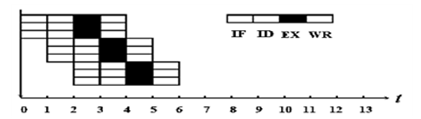
\includegraphics[width=4.37500in,height=1.22917in]{computerassets/bb2f406e57cb9867c61ecb280bd597b7.png}~

上图是超标量流水线的示意图,很明显,在每个时钟周期内同时发射了多条指令,当然这些同时执行需要多个不同的功能部件,通过这些部件的并行运行来提高指令的吞吐率,故B、C和D都是正确的叙述。超标量技术并没有采用更多的流水段个数,这是超流水线技术的做法,故A错误。
\end{solution}
